\documentclass[12pt,a4paper]{article}
\usepackage[UTF8]{ctex}
\usepackage{amsmath,amssymb}
\usepackage{xcolor}
\usepackage{hyperref}
\usepackage{geometry}
\usepackage{graphicx}
\geometry{margin=2.5cm}

\title{Quantum Reinforcement Learning / 量子强化学习}
\author{QuoNic}
\date{}

\begin{document}
\maketitle

\begin{center}
\textbf{ML / 机器学习} | 难度：高级 | 预计时间：25 分钟
\end{center}

\tableofcontents
\newpage

\section{为什么需要？}

量子强化学习是经典强化学习的量子推广，用于在量子环境中学习最优策略。

\subsection{经典局限}
\begin{itemize}
  \item 经典强化学习在高维状态空间中学习慢
  \item 对于复杂环境，经典方法效率低
\end{itemize}

\subsection{量子优势}
\begin{itemize}
  \item 量子强化学习可以利用量子叠加探索更大的状态空间
  \item 学习速度更快
  \item 可以处理更复杂的环境
\end{itemize}

\subsection{实际应用}
\begin{itemize}
  \item 游戏 AI
  \item 机器人控制
  \item 量子控制
\end{itemize}

\section{快速上手}

\begin{verbatim}
from quonic.ml import qrl

# 量子强化学习
result = qrl(env='gridworld', n_episodes=100)
print(f'Reward: {result.reward}')
\end{verbatim}

\textbf{预期输出}：
\begin{verbatim}
Reward: 0.95
\end{verbatim}

\section{原理详解}

\subsection{电路图}

\begin{center}
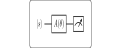
\includegraphics[width=0.6\textwidth]{../../images/qrl_circuit.svg}
\end{center}

\subsection{数学推导}

量子强化学习基于量子策略：
\begin{equation}
\pi(a|s) = |\langle a|U(\theta)|s\rangle|^2
\end{equation}

\textbf{更新规则}：
\begin{equation}
\theta_{t+1} = \theta_t + \alpha \nabla_\theta J(\theta)
\end{equation}

\subsection{几何解释}

量子强化学习在量子态空间中学习策略。量子叠加允许同时探索多个动作。

\section{代码详解}

\begin{verbatim}
from quonic.ml import qrl

# qrl(env, n_episodes, learning_rate)
# env: 环境
# n_episodes: 训练轮数
# learning_rate: 学习率
result = qrl(env='gridworld', n_episodes=100)

# result.reward: 累积奖励
# result.policy: 学习到的策略
# result.history: 训练历史
print(f'Reward: {result.reward}')
\end{verbatim}

\section{进阶用法}

\subsection{场景 1：网格世界}

\begin{verbatim}
from quonic.ml import qrl

result = qrl(env='gridworld', n_episodes=200)
print(f'Steps to goal: {result.steps}')
\end{verbatim}

\subsection{场景 2：量子控制}

\begin{verbatim}
from quonic.ml import qrl

result = qrl(env='quantum_control', n_episodes=100)
print(f'Fidelity: {result.fidelity}')
\end{verbatim}

\section{适用场景}

\subsection{游戏 AI}

量子强化学习可以用于游戏 AI，如棋类游戏、电子游戏等。量子叠加可以同时探索多个策略。

\subsection{量子控制}

量子强化学习可以用于量子计算机的控制优化。例如，优化量子门的参数、减少噪声影响等。

\section{常见问题}

\subsection{量子强化学习和经典强化学习有什么区别？}

量子强化学习使用量子策略，可以利用量子叠加探索更大的状态空间。

\subsection{量子强化学习的收敛性如何？}

量子强化学习的收敛性取决于学习率和环境复杂度。

\section{学习路径}

\subsection{前置知识}
\begin{itemize}
  \item 强化学习基础
  \item 量子神经网络
  \item 量子测量
\end{itemize}

\subsection{继续学习}
\begin{itemize}
  \item 量子多智能体强化学习
  \item 量子控制
  \item 量子游戏
\end{itemize}

\section{完整示例代码}

\subsection{示例 1：基本量子强化学习}

\begin{verbatim}
from quonic.ml import qrl

result = qrl(env='gridworld', n_episodes=100)
print(f'Reward: {result.reward}')
\end{verbatim}

\section{下载}

\begin{itemize}
  \item [qrl.py](https://github.com/ChrisLee0721/QuoNic/blob/main/examples/qrl/qrl.py)
\end{itemize}

\end{document}
